\chapter{Hardware setup}\label{ch:hardware}
In order to connect to the camera and the robot, a personal workstation has been used. Most of the time spent by our group was in the Robotics laboratory, where we worked and tested the ADEPT Cobra robot. We placed the camera inside the robot cell, above the blocks, such that we take images from the top. Such an image will allow us to efficiently determine the positions and orientations of the blocks. 

The phisical connections to the workstation were made through: 
\begin{itemize}
	\item Ethernet to the robot  
	\item USB to the camera 
\end{itemize}

\begin{figure}[hb]
\centering
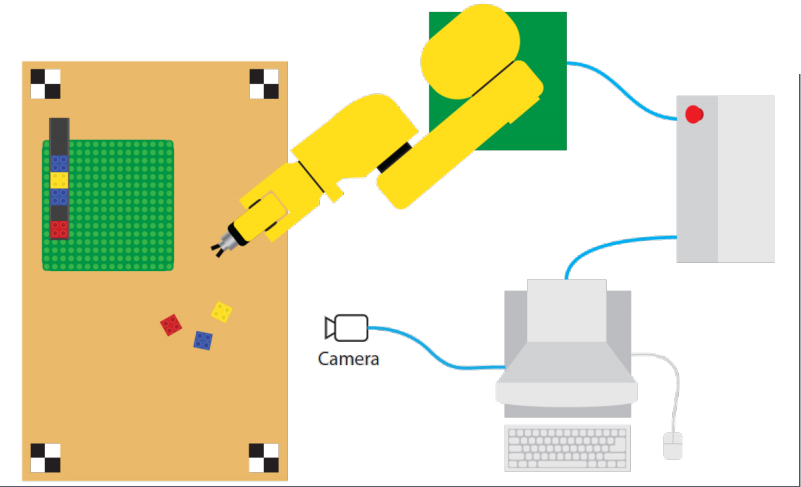
\includegraphics[width=4in]{figures/robotCellDesign.png}
\caption[robot Cell Design]
{An illustration of the hardware setup}
\end{figure}

A local computer with Windows XP runs the ADEPT Desktop program in order to control the robot. This computer is connected to a switch nearby and has a static IP. Thus, we take advantage of that by connecting our workstation to that switch through an Ethernet cable, such that we can connect to the ADEPT Desktop. Doing so we are able to communicate with the robot and using Matlab we can send commands to it. Regarding the camera, we have installed the webcam package in order to properly connect and use it. 
